\documentclass[11pt]{article}
% teacher_preamble.tex — shared preamble for the chalk-teaching TEACHER'S NOTES.
% These are standalone, instructor-facing lesson plans (article class), separate
% from the student lecture notes.  Compile each teaching/lecNN_teacher_notes.tex
% directly with pdfLaTeX.
\usepackage[T1]{fontenc}
\usepackage[utf8]{inputenc}
\usepackage[margin=1in]{geometry}
\usepackage{amsmath,amssymb,amsthm,mathtools}
\usepackage{braket}
\usepackage{bm}
\usepackage{graphicx}
\usepackage{enumitem}
\usepackage{xcolor}
\usepackage{tikz}
\usetikzlibrary{arrows.meta}
\usepackage{quantikz}
\usepackage[most]{tcolorbox}
\usepackage[colorlinks=true,linkcolor=blue,urlcolor=blue]{hyperref}

% ---- Notation macros (consistent with the course preamble.tex) ----
\newcommand{\R}{\mathbb{R}}
\newcommand{\C}{\mathbb{C}}
\newcommand{\N}{\mathbb{N}}
\newcommand{\Z}{\mathbb{Z}}
\newcommand{\E}{\mathbb{E}}
\newcommand{\Prob}{\mathbb{P}}
\newcommand{\Hilb}{\mathcal{H}}
\newcommand{\ii}{\mathrm{i}}
\newcommand{\dd}{\mathrm{d}}
\newcommand{\ee}{\mathrm{e}}
\DeclareMathOperator{\tr}{tr}
\DeclareMathOperator{\Tr}{Tr}
\DeclareMathOperator{\Var}{Var}
\DeclareMathOperator{\diag}{diag}
\newcommand{\norm}[1]{\left\lVert #1 \right\rVert}
\newcommand{\abs}[1]{\left\lvert #1 \right\rvert}
\newcommand{\bigo}{\mathcal{O}}
\newcommand{\id}{\mathbb{I}}
\newcommand{\dg}{^{\dagger}}
% quantikz also defines \proj (a circuit element we do not use); override it with our projector.
\let\proj\relax
\newcommand{\proj}[1]{\ket{#1}\!\bra{#1}}
\newcommand{\Xgate}{\mathsf{X}}
\newcommand{\Ygate}{\mathsf{Y}}
\newcommand{\Zgate}{\mathsf{Z}}
\newcommand{\Hgate}{\mathsf{H}}
\newcommand{\CNOT}{\mathrm{CNOT}}
\newcommand{\Uf}{U_f}

% ---- Theorem-like environments (numbered per section, article style) ----
\theoremstyle{definition}
\newtheorem{definition}{Definition}[section]
\newtheorem{example}[definition]{Example}
\theoremstyle{plain}
\newtheorem{theorem}[definition]{Theorem}
\newtheorem{lemma}[definition]{Lemma}
\newtheorem{proposition}[definition]{Proposition}
\theoremstyle{remark}
\newtheorem{remark}[definition]{Remark}

% ---- Teaching-specific structure ----
% Session block header with a time budget, e.g. \block{Qubits and the Bloch sphere}{45}
\newcommand{\block}[2]{%
  \bigskip\noindent
  \begin{tcolorbox}[colback=blue!6,colframe=blue!55!black,boxrule=0.6pt,arc=2pt,
    left=8pt,right=8pt,top=5pt,bottom=5pt]
  \textbf{\large #1}\hfill\textbf{[\,#2\,min]}
  \end{tcolorbox}}

% Board-plan cue: what to write/draw on the board.
\newtcolorbox{board}{colback=gray!8,colframe=gray!55!black,title={On the board},
  fonttitle=\bfseries\small,boxrule=0.5pt,arc=2pt,left=6pt,right=6pt,top=3pt,bottom=3pt}

% Graphic-demonstration cue (what to sketch).
\newcommand{\sketch}[1]{\par\smallskip\noindent{\color{teal}\textbf{Sketch:}} #1\par\smallskip}

% Optional / advanced material that may be skipped (but indicated).
\newtcolorbox{advanced}{colback=orange!7,colframe=orange!65!black,
  title={Advanced --- may be skipped (mention only)},
  fonttitle=\bfseries\small,boxrule=0.5pt,arc=2pt,left=6pt,right=6pt,top=3pt,bottom=3pt}

% Timing hint inline, e.g. \tmark{10} for a ~10-minute chunk.
\newcommand{\tmark}[1]{{\small\color{blue!55!black}(\,$\approx$#1\,min)}}

% In-class problem (numbered per section) and a teacher-facing answer.
\newtheorem{inclass}[definition]{In-class problem}
\newenvironment{answer}{\par\smallskip\noindent\textit{Answer.}\ }{\par\smallskip}

\title{\textbf{Lecture 2 --- Quantum Channels, Distances, and Statistical Estimates}\\[0.3em]\large Teacher's Notes (chalk, one 3$\times$45\,min meeting)}
\author{Course Instructor}
\date{}
\begin{document}
\maketitle

\noindent\textbf{How to use these notes.} This is a chalk-delivery lesson plan for
one three-hour meeting, split into three 45-minute blocks. Boxed \textsf{On the
board} panels give the exact equations and text to write; \textcolor{teal}{\textbf{Sketch}}
cues say what to draw; \tmark{n} markers pace each chunk. Work the derivations
\emph{live} at the board rather than reading them out. Each block has in-class
problems with teacher-facing answers---put the problem up, give students 3--6
minutes, then walk the solution. Orange \emph{Advanced} boxes are optional; mention
them only if time allows.

\medskip
\noindent\textbf{Learning goals (by the end of the meeting a student can):}
\begin{itemize}[leftmargin=1.4em,nosep]
  \item Explain why noise and subsystems force us past pure states, and write a channel in Kraus form $\mathcal E(\rho)=\sum_k E_k\rho E_k\dg$ with $\sum_k E_k\dg E_k=\id$.
  \item Give the Kraus operators of the bit-flip, phase-flip, depolarizing, and amplitude-damping channels, and show dephasing decays coherences as $\ee^{-t/T_2}$.
  \item Compute the trace distance and fidelity of two single-qubit states, interpret $T$ as the optimal one-shot distinguishing advantage, and use Fuchs--van de Graaf.
  \item Size a shot budget with Markov/Chebyshev/Hoeffding: $N=\bigo(\log(1/\delta)/\varepsilon^2)$ shots for additive error $\varepsilon$ at confidence $1-\delta$.
\end{itemize}

\medskip
\noindent\textbf{Prerequisites.} Lecture 1: qubits as unit vectors in $\C^2$, the
Born rule, the Bloch sphere, unitary gates $X,Y,Z,H,\CNOT$. Crucially the
\emph{density operator} $\rho=\sum_i p_i\proj{\psi_i}$ ($\rho\succeq0$, $\Tr\rho=1$),
introduced at the end of Lecture 1, and basic probability (mean, variance,
independence).

\medskip
\noindent\textbf{Materials.} Blackboard with room for a persistent ``cheat strip''
on one side (density-operator conditions, the Kraus completeness relation, the
Hoeffding shot count); \emph{colored chalk} (white for algebra, one color for
Bloch-ball pictures and axes, one for probabilities/error bars).

% =====================================================================
\block{Block 1 --- From mixed states to quantum channels}{45}
% =====================================================================
\noindent\emph{Objective:} noise and discarded subsystems force density operators;
a channel is the most general legal evolution of a density operator---a CPTP map---and
in practice it is a short list of Kraus operators. Dephasing then \emph{decays
coherence} exponentially.

\medskip
\noindent\textbf{Pacing:} why mixed states \tmark{8}; channel $=$ CPTP $=$ Kraus
\tmark{10}; example zoo \tmark{9}; in-class problem 1 \tmark{5}; dephasing
derivation \& Bloch sketch \tmark{8}; in-class problem 2 \tmark{5}.

\subsection*{1. Why we need mixed states \tmark{8}}
Open with the two reasons a state vector is not enough; keep them on the cheat strip.

\begin{board}
\textbf{Density operator.} $\rho\succeq0$, $\Tr\rho=1$. Pure: $\rho=\proj\psi$
($\Tr\rho^2=1$). Mixed: $\rho=\sum_i p_i\proj{\psi_i}$ ($\Tr\rho^2<1$).
\textbf{Two reasons we need it:}
\begin{itemize}
\item[(i)] \emph{Subsystems:} the state of half of an entangled pair is mixed
(partial trace of a pure whole).
\item[(ii)] \emph{Noise:} a device that is ``$X$ with prob.\ $1-p$, nothing with
prob.\ $p$'' produces a \emph{probabilistic mixture}, not a vector.
\end{itemize}
Born rule in this language: $\Prob(m)=\Tr(\proj m\rho)$; expectation
$\langle O\rangle=\Tr(O\rho)$.
\end{board}

Say aloud: a state vector answers ``which superposition?''; a density operator also
answers ``which \emph{classical} uncertainty am I in about the superposition?''
Interference lives in the \emph{off-diagonal} entries---remember that for the
dephasing derivation later.

\subsection*{2. A channel is a CPTP map, i.e.\ a Kraus sum \tmark{10}}
Do not belabor complete positivity---state it, give the one-line reason, then move to
the working definition (Kraus).

\begin{board}
\textbf{Channel (working definition).} A quantum channel $\mathcal E$ maps density
operators to density operators via the \emph{Kraus / operator-sum} form
\[
  \mathcal E(\rho)=\sum_k E_k\,\rho\,E_k\dg,\qquad
  \boxed{\ \sum_k E_k\dg E_k=\id\ }\ \text{(completeness).}
\]
The boxed relation is exactly trace preservation:
$\Tr\mathcal E(\rho)=\sum_k\Tr(E_k\rho E_k\dg)=\Tr\!\big(\rho\sum_k E_k\dg E_k\big)=\Tr\rho.$
\textbf{Formal name:} completely positive (CP) $+$ trace preserving (TP) $=$ CPTP.
\end{board}

One-line reason for the word \emph{completely}: mere positivity is not enough because
the input may be entangled with an untouched ancilla; the transpose map is positive
but sends the Bell state to something with a negative eigenvalue. State this, defer
the check to the student notes.

\begin{advanced}
Stinespring dilation: \emph{every} channel is a unitary on system$+$environment
followed by discarding the environment, $\mathcal E(\rho)=\Tr_R(V\rho V\dg)$ with
$V\dg V=\id$. ``All evolution is unitary once the box is big enough.'' Mention only;
full statement in the student notes. The picture: run a joint unitary $U$ on the
system $\rho$ together with a fresh environment $\ket0$, then throw the environment
away (trace it out --- here a meter, since discarding is a measurement we ignore):
\begin{center}
\begin{quantikz}
\lstick{$\rho$}   & \gate[2]{U} & \qw      & \rstick{$\mathcal E(\rho)$}\qw \\
\lstick{$\ket0$}  &             & \meter{} &
\end{quantikz}
\end{center}
\end{advanced}

\subsection*{3. The example zoo (memorize these Kraus operators) \tmark{9}}
\begin{board}
\textbf{Bit-flip:} $E_0=\sqrt p\,\id$, $E_1=\sqrt{1-p}\,X$; $\ \mathcal E(\rho)=p\rho+(1-p)X\rho X$.\\
\textbf{Phase-flip (dephasing):} $E_0=\sqrt p\,\id$, $E_1=\sqrt{1-p}\,Z$; $\ \mathcal E(\rho)=p\rho+(1-p)Z\rho Z$.\\
\textbf{Depolarizing:} $\mathcal E(\rho)=p\,\rho+(1-p)\dfrac{\id}{2}$ (one qubit); isotropic noise.\\
\textbf{Amplitude damping} ($\ket1\to\ket0$ with prob.\ $\gamma$):
\[
  E_0=\begin{pmatrix}1&0\\0&\sqrt{1-\gamma}\end{pmatrix},\quad
  E_1=\begin{pmatrix}0&\sqrt\gamma\\0&0\end{pmatrix},\quad
  E_0\dg E_0+E_1\dg E_1=\id.
\]
\end{board}

Contrast to say aloud: bit-flip/phase-flip/depolarizing are \emph{unital}
($\mathcal E(\id)=\id$, center of the Bloch ball fixed); amplitude damping is
\emph{not}---it drags every state toward $\ket0$ (energy loss).

\begin{inclass}[Phase-flip Kraus operators check]\label{ic:pf}
Write the phase-flip Kraus operators and verify $\sum_k E_k\dg E_k=\id$. Then compute
$\mathcal E(\proj{+})$ for $p=\tfrac12$ and say what happened to the coherence.
\end{inclass}
\begin{answer}
$E_0=\sqrt p\,\id$, $E_1=\sqrt{1-p}\,Z$. Since $\id\dg\id=\id$ and $Z\dg Z=Z^2=\id$,
$\sum_k E_k\dg E_k=p\,\id+(1-p)\id=\id$. \checkmark\ \ With
$\proj{+}=\tfrac12\big(\begin{smallmatrix}1&1\\1&1\end{smallmatrix}\big)$ and $p=\tfrac12$:
$Z\proj{+}Z=\tfrac12\big(\begin{smallmatrix}1&-1\\-1&1\end{smallmatrix}\big)$, so
$\mathcal E(\proj+)=\tfrac12\proj++\tfrac12 Z\proj+ Z=\tfrac12\big(\begin{smallmatrix}1&0\\0&1\end{smallmatrix}\big)=\tfrac12\id$.
The off-diagonal (coherence) is wiped out; the diagonal (populations $\tfrac12,\tfrac12$) survives.
\end{answer}

\subsection*{4. Decoherence: dephasing decays the coherence \tmark{8}}
This is the physics payoff. Derive the exponential decay live.

\begin{board}
Write $\rho=\big(\begin{smallmatrix}\rho_{00}&\rho_{01}\\ \rho_{10}&\rho_{11}\end{smallmatrix}\big)$.
Because $Z\ket0\!\bra1 Z=-\ket0\!\bra1$, $Z\rho Z$ flips the sign of the off-diagonals only:
\[
  \mathcal E_{\mathrm{pf}}(\rho)=p\rho+(1-p)Z\rho Z
  =\begin{pmatrix}\rho_{00}&(2p-1)\rho_{01}\\ (2p-1)\rho_{10}&\rho_{11}\end{pmatrix}.
\]
One time step multiplies the coherence by $2p-1\in[-1,1]$; populations untouched.
Set $2p-1=\ee^{-\Delta t/T_2}$; after time $t=n\Delta t$,
\[
  \boxed{\ \rho_{01}(t)=\ee^{-t/T_2}\,\rho_{01}(0)\ }.
\]
As $t\to\infty$, $\rho\to\diag(\rho_{00},\rho_{11})$: a superposition becomes a
classical mixture \emph{without anyone measuring}.
\end{board}

\sketch{Bloch ball CONTRACTING. Draw the unit sphere; a pure state as an arrow of
length $1$ to the surface. Under \emph{dephasing}: the ball collapses toward the
$z$-axis (an ellipsoid squashed in $x,y$), so equatorial states shrink inward, the
poles $\ket0,\ket1$ stay fixed. Under \emph{depolarizing}: the whole ball shrinks
uniformly, $\vec r\mapsto p\,\vec r$, toward the center $\tfrac12\id$. Say aloud:
loss of coherence $=$ loss of Bloch-vector length $=$ the arrow retreating from the
surface into the interior.}

\noindent Reference picture to reproduce on the board --- the unit Bloch ball (solid
circle) contracting to a smaller region (dashed) as coherence is lost: under
\emph{depolarizing} it shrinks to a smaller ball $\vec r\mapsto p\,\vec r$; under
\emph{dephasing} it squashes to an ellipse flattened in the equatorial ($x,y$)
directions while the poles $\ket0,\ket1$ stay put:
\begin{center}
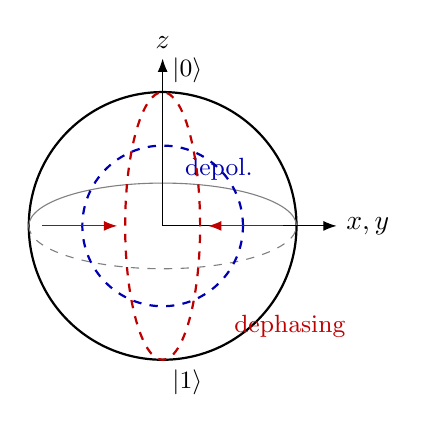
\begin{tikzpicture}[scale=1.7,>=Latex]
  % unit Bloch ball
  \draw[thick] (0,0) circle (1);
  \draw[dashed,gray] (-1,0) arc (180:360:1 and 0.32);
  \draw[gray] (1,0) arc (0:180:1 and 0.32);
  % axes
  \draw[->] (0,0) -- (0,1.25) node[above] {$z$};
  \draw[->] (0,0) -- (1.3,0) node[right] {$x,y$};
  \node[above right] at (0,1) {\small$\ket0$};
  \node[below right] at (0,-1) {\small$\ket1$};
  % depolarizing: smaller concentric ball
  \draw[blue!70!black,thick,dashed] (0,0) circle (0.6);
  \node[blue!70!black] at (0.42,0.42) {\small depol.};
  % dephasing: ellipse squashed in x,y (narrow horizontally, poles fixed)
  \draw[red!75!black,thick,dashed] (0,0) ellipse (0.28 and 1);
  \node[red!75!black,align=left] at (0.95,-0.75) {\small dephasing};
  % arrows showing contraction
  \draw[->,red!75!black] (0.9,0) -- (0.34,0);
  \draw[->,red!75!black] (-0.9,0) -- (-0.34,0);
\end{tikzpicture}
\end{center}

\begin{inclass}[Depolarizing shrinks the Bloch vector]\label{ic:depol}
Write a one-qubit state as $\rho=\tfrac12(\id+\vec r\cdot\vec\sigma)$. Show the
depolarizing channel $\mathcal E(\rho)=p\rho+(1-p)\tfrac{\id}2$ sends $\vec r\mapsto p\,\vec r$.
\end{inclass}
\begin{answer}
$\mathcal E(\rho)=p\cdot\tfrac12(\id+\vec r\cdot\vec\sigma)+(1-p)\tfrac12\id
=\tfrac12\big(\id+p\,\vec r\cdot\vec\sigma\big)$. Matching to
$\tfrac12(\id+\vec r'\cdot\vec\sigma)$ gives $\vec r'=p\,\vec r$: the Bloch vector
shrinks by the factor $p$ toward the center, exactly the uniform contraction in the
sketch. (At $p=0$ every state collapses to $\tfrac12\id$.)
\end{answer}

% =====================================================================
\block{Block 2 --- Telling states apart: distances}{45}
% =====================================================================
\noindent\emph{Objective:} how different are two states, \emph{operationally}? Trace
distance $=$ best single-shot distinguishing advantage; fidelity $=$ overlap; the two
are tied by Fuchs--van de Graaf. For one qubit, $T=$ half the Bloch-vector distance.

\medskip
\noindent\textbf{Pacing:} trace distance \& operational meaning \tmark{10}; in-class
problem 1 \tmark{5}; single-qubit formula $T=\tfrac12\abs{\vec r_1-\vec r_2}$
derivation \& sketch \tmark{10}; fidelity \& Fuchs--van de Graaf \tmark{10};
in-class problem 2 \tmark{6}; advanced (diamond norm) \tmark{4}.

\subsection*{1. Trace distance and what it means \tmark{10}}
\begin{board}
\textbf{Trace norm:} $\norm A_1=\Tr\abs A=\sum_i\sigma_i(A)$ (sum of singular values).
\textbf{Trace distance:}
\[
  T(\rho,\sigma)=\tfrac12\norm{\rho-\sigma}_1\in[0,1].
\]
\textbf{Operational meaning.} One copy, guess $\rho$ vs.\ $\sigma$ (prior $\tfrac12$
each) with the best measurement:
\[
  p_{\mathrm{success}}=\tfrac12\big(1+T(\rho,\sigma)\big),\qquad
  T=\max_{0\preceq M\preceq\id}\Tr[M(\rho-\sigma)].
\]
$T=0$: identical, coin-flip guess. $T=1$: perfectly distinguishable in one shot.
\end{board}

Sketch the argument aloud (do not fully prove): split $\rho-\sigma=\Delta_+-\Delta_-$
into positive/negative parts; the optimal measurement is the projector $P$ onto the
positive part, and $\Tr[P(\rho-\sigma)]=\Tr\Delta_+=T$. Moral: trace distance is a
\emph{promise about every measurement at once}---no experiment separates the two by
more than $T$.

\begin{inclass}[Trace distance of $\proj0$ and $\proj+$]\label{ic:tdist}
Compute $T(\proj0,\proj+)$ with $\ket+=\tfrac1{\sqrt2}(\ket0+\ket1)$. What is the best
single-shot success probability?
\end{inclass}
\begin{answer}
$\rho-\sigma=\proj0-\proj+=\big(\begin{smallmatrix}1&0\\0&0\end{smallmatrix}\big)
-\tfrac12\big(\begin{smallmatrix}1&1\\1&1\end{smallmatrix}\big)
=\tfrac12\big(\begin{smallmatrix}1&-1\\-1&-1\end{smallmatrix}\big)$. This is
Hermitian traceless; eigenvalues $\pm\lambda$ with
$\lambda=\tfrac12\sqrt{1^2+1^2}=\tfrac1{\sqrt2}$. So $\norm{\rho-\sigma}_1=2\lambda=\sqrt2$
and $T=\tfrac12\sqrt2=\tfrac1{\sqrt2}\approx0.707$. Best success
$p=\tfrac12(1+\tfrac1{\sqrt2})\approx0.854$.
\end{answer}

\subsection*{2. Single-qubit formula: $T=\tfrac12\abs{\vec r_1-\vec r_2}$ \tmark{10}}
Derive the clean geometric formula---it makes trace distance a \emph{ruler} on the
Bloch ball.

\begin{board}
\textbf{Claim.} For $\rho_j=\tfrac12(\id+\vec r_j\cdot\vec\sigma)$,
$\ T(\rho_1,\rho_2)=\tfrac12\abs{\vec r_1-\vec r_2}$.
\textbf{Derivation.} $\rho_1-\rho_2=\tfrac12(\vec r_1-\vec r_2)\cdot\vec\sigma$.
For any real vector $\vec a$, $\vec a\cdot\vec\sigma$ has eigenvalues $\pm\abs{\vec a}$
(since $(\vec a\cdot\vec\sigma)^2=\abs{\vec a}^2\id$). With $\vec a=\tfrac12(\vec r_1-\vec r_2)$,
\[
  \norm{\rho_1-\rho_2}_1=2\cdot\tfrac12\abs{\vec r_1-\vec r_2}=\abs{\vec r_1-\vec r_2},
  \quad\Rightarrow\quad T=\tfrac12\abs{\vec r_1-\vec r_2}.
\]
\end{board}

Cross-check with In-class~\ref{ic:tdist}: $\ket0\!\to\!\vec r=(0,0,1)$,
$\ket+\!\to\!\vec r=(1,0,0)$; $\abs{\vec r_1-\vec r_2}=\sqrt2$, half is $\tfrac1{\sqrt2}$. \checkmark

\sketch{Two points in the Bloch ball (tips of $\vec r_1,\vec r_2$). Draw the chord
between them; $T$ is HALF its length. Then draw the optimal distinguishing
measurement as a \emph{plane} perpendicular to $\vec r_1-\vec r_2$ and through the
center: measure along $\vec r_1-\vec r_2$, guess whichever side the outcome lands.
Antipodal points ($\ket0$ vs.\ $\ket1$) give the maximum $T=1$.}

\subsection*{3. Fidelity and Fuchs--van de Graaf \tmark{10}}
\begin{board}
\textbf{Fidelity.} $F(\rho,\sigma)=\Tr\sqrt{\rho^{1/2}\sigma\rho^{1/2}}\in[0,1]$;
$F=1\iff\rho=\sigma$. Pure states: $F(\proj\psi,\proj\varphi)=\abs{\braket{\psi|\varphi}}$.
\textbf{Fuchs--van de Graaf (ties $F$ and $T$):}
\[
  1-F\ \le\ T\ \le\ \sqrt{1-F^2}.
\]
Small-error reading ($F=\cos\theta$, $\theta$ small): $\tfrac12\theta^2\lesssim T\lesssim\theta$.
\end{board}

Why keep both: $T$ directly bounds measurement statistics (error propagation), $F$ is
often the easier lab quantity (swap test). Converting infidelity $1-F=\varepsilon$
gives $T\le\sqrt{2\varepsilon}$---the usual bridge.

\begin{inclass}[Fidelity of $\proj0,\proj+$ and the FvdG check]\label{ic:fid}
Compute $F(\proj0,\proj+)$ and check both Fuchs--van de Graaf inequalities against the
$T=\tfrac1{\sqrt2}$ from In-class~\ref{ic:tdist}.
\end{inclass}
\begin{answer}
Both pure, so $F=\abs{\braket{0|+}}=\tfrac1{\sqrt2}\approx0.707$. Lower bound:
$1-F=1-\tfrac1{\sqrt2}\approx0.293\le0.707=T$. \checkmark\ \ Upper bound:
$\sqrt{1-F^2}=\sqrt{1-\tfrac12}=\tfrac1{\sqrt2}\approx0.707=T$: the upper bound is
\emph{attained} (equality always holds for pure states). \checkmark
\end{answer}

\begin{advanced}
\textbf{Channels: the diamond norm.} To compare two channels one takes
$\norm{\mathcal E-\mathcal F}_\diamond=\sup_k\sup_{\norm X_1\le1}\norm{(\mathcal E-\mathcal F)\otimes\mathcal I_k)(X)}_1$---the
stabilized version, allowing an entangled reference qubit (same reason CP beats
positivity). It is subadditive, so per-gate error $\le\eta$ over $m$ gates gives
total $\le2m\eta$ (error grows linearly in depth). For unitaries
$\norm{\mathcal U-\mathcal V}_\diamond\le2\norm{U-V}_\infty$. Mention only.
\end{advanced}

% =====================================================================
\block{Block 3 --- Statistics: reading answers off a quantum computer}{45}
% =====================================================================
\noindent\emph{Objective:} measurements are random, so every number is an estimate
from samples. Markov $\to$ Chebyshev $\to$ Hoeffding give the error bars, and
Hoeffding fixes the shot budget $N=\bigo(\log(1/\delta)/\varepsilon^2)$.

\medskip
\noindent\textbf{Pacing:} sampling setup \tmark{6}; Markov \& Chebyshev (proofs)
\tmark{10}; Hoeffding \& the shot-count derivation \tmark{12}; in-class problem 1
\tmark{5}; amplification \& in-class problem 2 \tmark{8}; advanced (Fisher/CRB)
\tmark{4}.

\subsection*{1. Why statistics at all \tmark{6}}
\begin{board}
Measuring $O$ on $\rho$ returns a random outcome; only $\langle O\rangle=\Tr(O\rho)$
is deterministic, and we see it only \emph{on average}. Estimate it by $N$ shots:
$\bar X=\tfrac1N\sum_i X_i$, $\E[\bar X]=\langle O\rangle$. Question: how large must
$N$ be so that $\abs{\bar X-\langle O\rangle}\le\varepsilon$ with confidence $1-\delta$?
\end{board}
Frame the block: three inequalities, each stronger and needing more assumptions
(nonneg $\to$ finite variance $\to$ bounded), then read the shot count off the last.

\noindent A concrete example of ``a number read off from statistics'' is the
\emph{Hadamard test}, the workhorse for estimating $\mathrm{Re}\braket{\psi|U|\psi}$:
an ancilla in $\ket0$ is put in superposition by $H$, controls $U$ on the system
$\ket\psi$, is closed by a second $H$, and measured. The measurement is Bernoulli,
so its bias is exactly the quantity we want --- and the shot budget below fixes how
many repetitions we need:
\begin{center}
\begin{quantikz}
\lstick{$\ket0$}    & \gate{H} & \ctrl{1} & \gate{H} & \meter{} & \cw \\
\lstick{$\ket\psi$} & \qw      & \gate{U} & \qw      & \qw      &
\end{quantikz}
\end{center}
\noindent Here $\Prob(0)=\tfrac12\big(1+\mathrm{Re}\braket{\psi|U|\psi}\big)$, so
$\langle Z_{\mathrm{anc}}\rangle=\mathrm{Re}\braket{\psi|U|\psi}$: estimating a single
Bernoulli bias to additive error $\varepsilon$ is exactly the shot-budget problem of
this block.

\subsection*{2. Markov, then Chebyshev \tmark{10}}
\begin{board}
\textbf{Markov.} $X\ge0,\ t>0\ \Rightarrow\ \Prob(X\ge t)\le\E[X]/t$.
\emph{Proof:} $X\ge t\,\mathbf 1_{X\ge t}$ pointwise; take $\E$:
$\E[X]\ge t\,\Prob(X\ge t)$.\\[2pt]
\textbf{Chebyshev.} $\Prob(\abs{X-\E X}\ge t)\le\Var(X)/t^2$.
\emph{Proof:} apply Markov to $(X-\E X)^2\ge0$ at level $t^2$:
$\Prob((X-\E X)^2\ge t^2)\le\E[(X-\E X)^2]/t^2=\Var(X)/t^2$.
\end{board}
Emphasize: Chebyshev is Markov applied to the squared deviation. Its tail decays only
\emph{polynomially} ($1/t^2$)---fine, but for many shots we can do exponentially better.

\begin{inclass}[Chebyshev shot count]\label{ic:cheb}
A single shot $X_i\in\{0,1\}$ has mean $p$, variance $p(1-p)\le\tfrac14$. Using
Chebyshev on $\bar X_N$ (variance $p(1-p)/N$), how many shots guarantee
$\Prob(\abs{\bar X_N-p}\ge\varepsilon)\le\delta$ in the worst case?
\end{inclass}
\begin{answer}
$\Prob(\abs{\bar X_N-p}\ge\varepsilon)\le\dfrac{p(1-p)}{N\varepsilon^2}\le\dfrac{1}{4N\varepsilon^2}$.
Set $\le\delta$: $N\ge\dfrac{1}{4\varepsilon^2\delta}$. Note the \emph{$1/\delta$}
confidence dependence---Hoeffding will improve this to $\log(1/\delta)$.
\end{answer}

\subsection*{3. Hoeffding and the shot budget \tmark{12}}
\begin{board}
\textbf{Hoeffding (Bernoulli form).} For i.i.d.\ $X_i\in\{0,1\}$ with mean $p$,
\[
  \Prob\!\big(\abs{\bar X_N-p}\ge\varepsilon\big)\ \le\ 2\exp(-2N\varepsilon^2).
\]
\textbf{Shot budget.} Set RHS $=\delta$ and solve for $N$:
\[
  2\ee^{-2N\varepsilon^2}=\delta
  \ \Rightarrow\ 2N\varepsilon^2=\log\tfrac2\delta
  \ \Rightarrow\ \boxed{\ N\ \ge\ \dfrac{\log(2/\delta)}{2\varepsilon^2}
  =\bigo\!\Big(\dfrac{\log(1/\delta)}{\varepsilon^2}\Big)\ }.
\]
\end{board}
The $N=\Theta(\varepsilon^{-2})$ scaling is the \emph{standard quantum limit}: halving
the error \emph{quadruples} the cost. And confidence is cheap---$\log(1/\delta)$, not
$1/\delta$ (contrast In-class~\ref{ic:cheb}).

\sketch{Shots-vs-error curve. Axes: horizontal $\varepsilon$, vertical $N$. Plot
$N\propto1/\varepsilon^2$, a steep decay: mark $\varepsilon=0.1\Rightarrow N\!\sim\!$
hundreds, $\varepsilon=0.01\Rightarrow N\!\sim\!$ tens of thousands. Second small
panel: $N$ vs.\ $\log(1/\delta)$ as a gentle straight line---``paying for confidence
is cheap, paying for precision is not.''}

\begin{inclass}[How many shots?]\label{ic:shots}
Estimate a probability to $\varepsilon=0.01$ with confidence $1-\delta=0.95$. Give the
Hoeffding shot count.
\end{inclass}
\begin{answer}
$\delta=0.05$, so $N\ge\dfrac{\log(2/0.05)}{2(0.01)^2}=\dfrac{\ln 40}{2\cdot10^{-4}}
=\dfrac{3.689}{0.0002}\approx1.84\times10^4$. So about $18{,}500$ shots. (Doubling
precision to $\varepsilon=0.005$ would quadruple this to $\sim74{,}000$.)
\end{answer}

\subsection*{4. Amplification: cheap confidence \tmark{8}}
\begin{board}
\textbf{Majority vote.} One run correct with prob.\ $p>\tfrac12$. Take majority of $N$
runs; wrong only if correct count $S\le N/2$. Hoeffding:
\[
  \Prob(S\le N/2)\le\exp\!\big(-2(p-\tfrac12)^2N\big)\le\delta
  \ \Rightarrow\ N\ge\frac{\log(1/\delta)}{2(p-\tfrac12)^2}.
\]
\emph{Median-of-means} does the same for real-valued estimates. Confidence costs only
$\log(1/\delta)$ repetitions.
\end{board}

\begin{inclass}[Majority-vote runs]\label{ic:maj}
A subroutine is correct with $p=0.6$ per run. How many runs $N$ make the majority
correct with probability $\ge1-\delta$, $\delta=10^{-3}$? Why is the $\delta$
dependence logarithmic?
\end{inclass}
\begin{answer}
$p-\tfrac12=0.1$, so $N\ge\dfrac{\log(1/\delta)}{2(0.1)^2}=\dfrac{\ln 1000}{0.02}
=\dfrac{6.908}{0.02}\approx345$; take $N=346$ (round up, even). Logarithmic because the
failure probability decays \emph{exponentially} in $N$ (independent runs, Hoeffding),
so inverting $\ee^{-cN}\le\delta$ gives $N\ge\log(1/\delta)/c$.
\end{answer}

\begin{advanced}
\textbf{Lower bound: Fisher information \& Cram\'er--Rao.} The shot counts above are
\emph{upper} bounds. The matching lower bound is $\Var(\hat\theta)\ge1/(N\,I_F(\theta))$
with Fisher information $I_F(\theta)=\E[(\partial_\theta\log P)^2]$; for a biased coin
$I_F(p)=1/(p(1-p))$, so $\Var(\hat p)\ge p(1-p)/N$ and the sample mean is
\emph{efficient}. Optimizing the measurement gives the quantum Fisher information and,
for an $N$-fold-entangled probe, the \emph{Heisenberg limit} $\Var\sim1/N^2$---the
$\varepsilon^{-2}\to\varepsilon^{-1}$ speedup realized by quantum phase estimation
(Lecture 4). Mention only; point to Lecture 4.
\end{advanced}

\end{document}
